In this chapter, we will use the results from \chpt\ to calculate the thermodynamic properties of our system, such as pressure and energy density, and study the phase diagram of \chpt.
We follow the procedure used in~\autocite{adhikariTwoflavorChiralPerturbation2019,martinariaTwoflavorChiralPerturbation2020}.

\section{Free energy in a homogenous system}
In our case, we are working with a homogenous system, in which we may write the free energy as $F = V\Eff$, where $\Eff$ is the \emph{free energy density}.
We use the grand canonical ensemble, so this is the grand canonical free energy, also called the grand canonical potential.
It is related to the partition function of statistical mechanics, $\mathcal{Z}$, by
%
\begin{equation}
    \Eff = - \frac{1}{V \beta} \ln \mathcal{Z}.
\end{equation}
%
Here, $V$ is the volume, and $\beta = 1/T$ is inverse temperature.
Using imaginary-time formalism for thermal field theory, described in \autoref{appendix: thermal field theory}, we find that the partition function is given by the path integral of the \emph{Euclidean} Lagrange density, as shown in equation \autoref{free scalar result 2}.
In the zero temperature limit  $\beta \rightarrow \infty$, the partition function is related to the generating functional $Z = Z[j]$, as described in \autoref{section: path integral}, by a Wick rotation.
The free energy density at zero temperature is therefore
%
\begin{equation}
    \Eff = \frac{i}{VT} \ln Z,
\end{equation}
%
where $VT$ is the volume of space-time.
As we found in \autoref{1PI effective action}, this equals the effective potential in the ground state.
In \autoref{section: effective action}, we found an explicit formula for this to one-loop order, \autoref{effective potential}.
In \autoref{appendix: consisten expansion}, we show how to expand free energy density and other thermodynamic quantities in a self-consistent way.

We are after the equation of state, which the free energy density will give us access to.
The free energy is defined as
%
\begin{equation}
    \label{thermodynamic free energy}
    F(T, V, \mu_I) = U - TS - {\sum}_i \mu_i Q_i, 
    \quad \dd 
    F = - S \dd T - p \dd V - {\sum}_i Q_i \dd \mu_i.
\end{equation}
%
Here, $U$ is the energy and $S$ the entropy.
$Q_i$ are conserved charges, in our case the isospin and strangeness charge, and $\mu_i$ their corresponding chemical potentials.
In our case, all results are for $T = 0$.
From \autoref{thermodynamic free energy}, the pressure is given by
%
\begin{equation}
    \label{pressure form free energy}
    p = - \left(\pdv{F}{V}\right)_{T, \mu} = - \Eff.
\end{equation}
%
The total charges are proportional to volume, which means that the corresponding densities are
%
\begin{equation}
    n_i = \frac{Q_i}{V} = - \frac{1}{V} \left(\pdv{F}{\mu_i}\right)_{T, V,\mu\neq\mu_i}
    = - \pdv{\Eff}{\mu_i}, \quad i = I, S.
\end{equation}
%
From \autoref{thermodynamic free energy} we get the energy density, $u = U/V$, at $T = 0$, is given by
%
\begin{equation}
    \label{energy density form pressure and isospin}
    u(\mu_I) = -p(\mu_i) + {\sum }_i\mu_i n_i(\mu_i),
\end{equation}



\section{Leading order analysis}

The leading order contribution to free energy is given by the static Lagrangian, to first order in Weinberg's power counting scheme.
We start by assuming $e = 0$, i.e., no electromagnetic interactions.
We thus get the leading order contribution to the free energy density from \autoref{static three-flavor lagrangian}, and it is
%
\begin{equation}
    \Eff 
    = 
    - \frac{1}{2} f^2
    \left(
        \mu_I^2 \sin^2\alpha
        + 2\bar m \cos\alpha
        + m_S
    \right).
\end{equation}
%
The parameter $\alpha$ is determined by minimizing $\Eff$ for a given value of $\mu_I$,
%
\begin{equation}
    \pdv{\Eff}{\alpha} = f^2 \left(\bar m^2 - \mu_I^2 \cos \alpha\right) \sin\alpha = 0.
\end{equation}
%
This gives an explicit formula for $\alpha$ in terms of $\mu_I$.
As long as the chemical potential is lower than the critical value $\mu_I^c = \bar m$, the only solution to this equation is $\alpha = 0$.
As the chemical potential reaches this critical value, the system undergoes a phase transition from the vacuum phase to the \emph{pion condensate} phase.
In this new phase, the solution is
%
\begin{align}
    \label{alpha as function of mu lowest order}
    \cos \alpha = \frac{\bar m^2}{\mu_I^2}.
\end{align}
%
We introduce a dimensionless variable $x^2 = \cos\alpha = \bar m^2 / \mu_I^2$.
This variable has the domain $[0, 1]$, and $\cos \alpha = x^2$ implies that $\sin^2 \alpha = 1 - x^4$.
Substituting the dimensionless variable into the free energy density, we get 
%
\begin{equation}
    \Eff = - \frac{u_0}{2} \left( x^2 + \frac{1}{x^2} \right) +\const
\end{equation}
%
We have introduced the characteristic energy density $u_0 = \bar m^2 f^2$.
As we found in the last section, the pressure is given by negative the free energy density, normalized to $\mu_I = \bar m$, or $x = 1$.
We choose $p_0 = u_0$, so the dimensionless pressure is
%
\begin{equation}
    \label{pressure leading order chpt}
    \tilde p = -\frac{1}{p_0} \left(\Eff - \Eff_{x=1}\right) 
    % = \frac{1}{2} \left( x^2 + \frac{1}{x^2} - 2 \right).
    = \frac{1}{2} \left(x - \frac{1}{x}\right)^2.
\end{equation}
%
The charge density corresponding to a chemical potential is given by minus the derivative of the free energy with respect to that chemical potential. 
We must, however, not assume any dependence of $\alpha$ on $\mu_I$ when taking this derivative.
The isospin density k is
%
\begin{equation}
    n_I = -\pdv{\Eff}{\mu_I} = \mu_I^2 \sin^2 \alpha 
    = 
    \frac{u_0}{\mu_I} \left(\frac{1}{x^2} - x^2\right),
\end{equation}
%
while the strangeness is zero.
With this, the dimensionless energy density at $T = 0$ is
%
\begin{equation}
    \label{energy density leading order chpt}
    \tilde u = - \tilde p + \frac{\mu_I n_I}{u_0}
    = \frac{1}{2} \left( 2 + \frac{1}{x^2} - 3 x^2\right).
\end{equation}
% 
The ratio of pressure to energy density is
%
\begin{equation} 
    \label{pressure energy ratio leading order chpt}
    \frac{p}{u} = \frac{1- x^2}{1+3x^2},
\end{equation}
%
which matches earlier results~\autocite{sonQCDFiniteIsospin2001}.
In the ultrarelativistic limit, where $\mu_I \rightarrow \infty$ and thus $x \rightarrow 0$, we get $p / u = 1$, or $u_\text{ur} = p$.
The non-relativistic limit is $\mu_I^2 = m_\pi^2(1 + \epsilon)$ and thus $x^{-2} = 1 + \epsilon$, $\epsilon \ll 1$.
With this we get $\tilde p = \epsilon^2 / 2 $, and $\tilde u = 2\epsilon$, so the equation of state is $\tilde u_\text{nr} = \sqrt 8 \sqrt{\tilde p}$.
The isospin density, and thus the pion number density, is $n_I = 2 \frac{u_0}{\bar m} \epsilon$, and we can therefore write the energy density in this limit as $u = \bar m n_I + \Oh(\epsilon^2)$.
The energy density is thus dominated by the rest mass as $\epsilon \rightarrow 0$, as we expect from the non-relativistic limit.
\autoref{fig: equation of state pions} shows the equation of state in two different regimes and compares it with the ultrarelativistic and non-relativistic limit.

\begin{figure}[h]
    \centering
    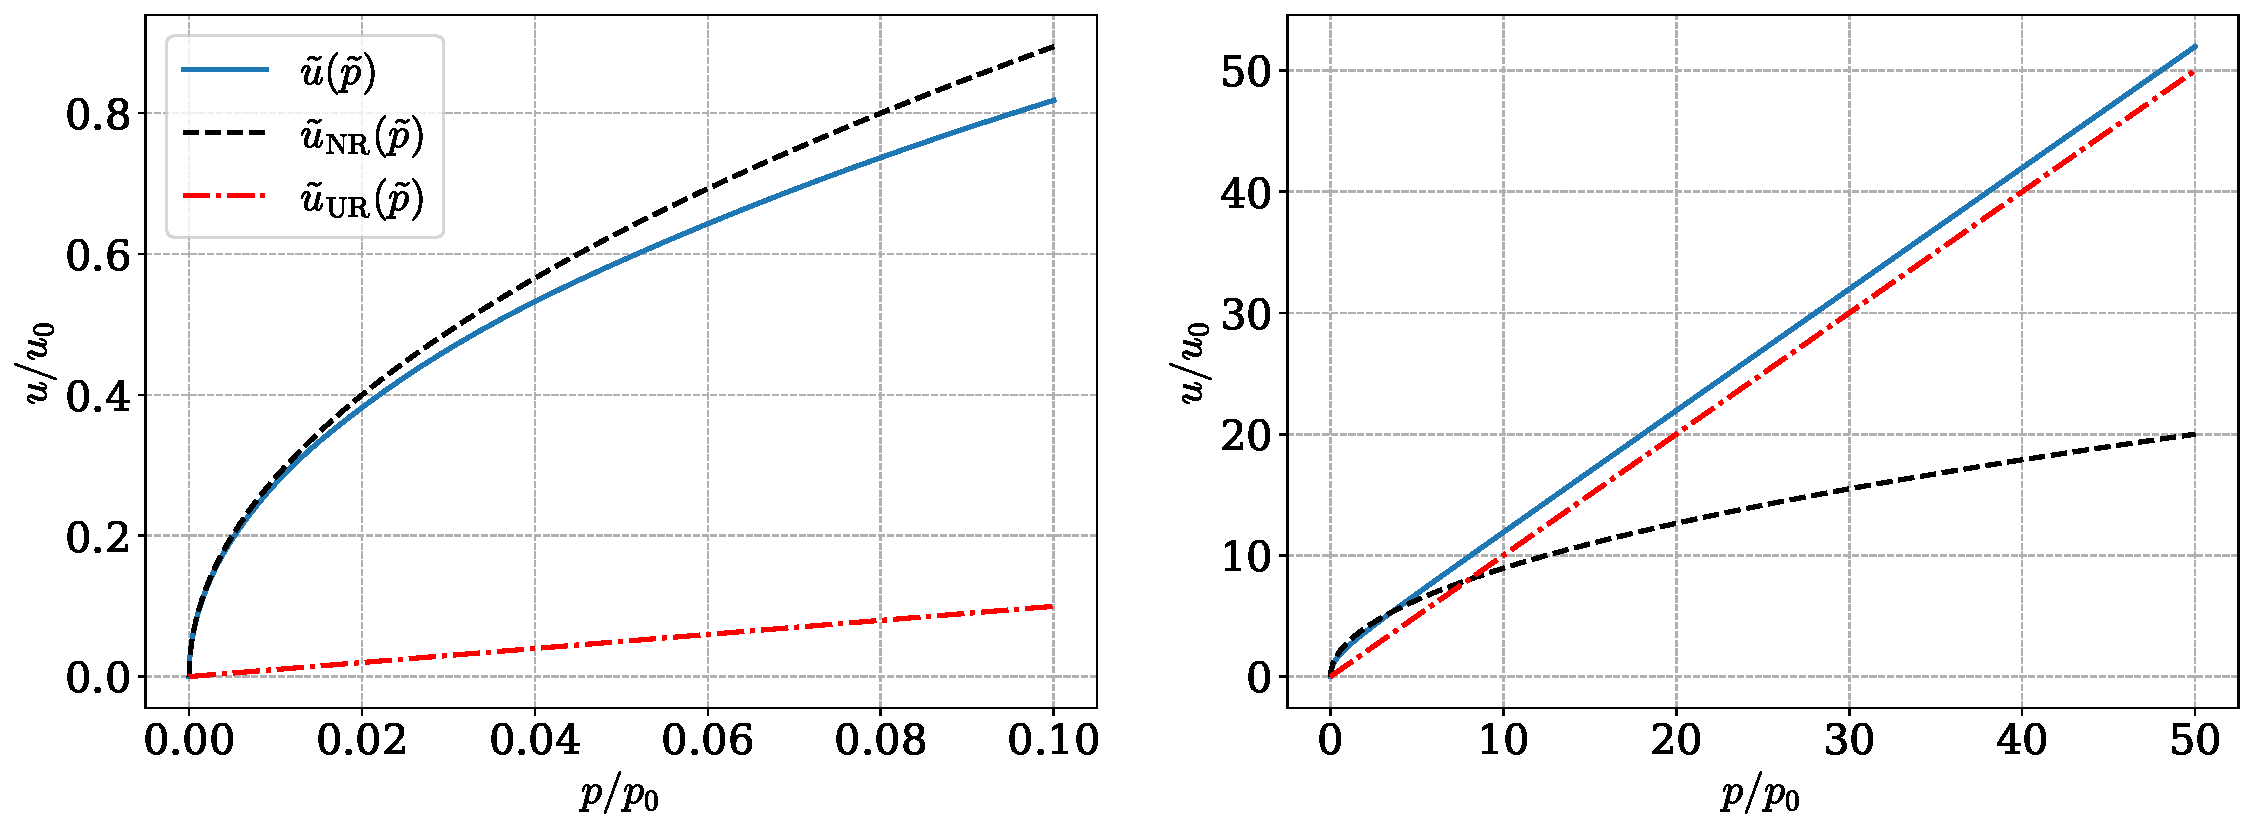
\includegraphics[width=0.95\textwidth]{../scripts/figurer/pion_star/pion_eos.pdf}
    \caption{
        The leading order equation of state from two-flavor chiral perturbation theory, in two different regimes.
        The full equation is shown as a solid line, and is compared to the ultrarelativistic and non-relativistic limit, shown as dashed lines. 
        The $y$-axis shows the energy density normalized to $u_0$, $x$-axis shows the pressure normalized to $p_0$.
        We have chosen $p_0 = u_0$.
    }
    \label{fig: equation of state pions}
\end{figure}



\subsection{Including electromagnetism}
\label{subsection: including electromagnetism lo eos}


From \autoref{static lagragniang three-flavor EM}, the free energy density, including electromagnetic interactions, is
%
\begin{equation}
    \Eff =
    - \frac{1}{2} f^2
    \left(
        \mu_I^2 \sin^2\alpha + 2 \bar m^2\cos\alpha 
        + \Delta m_\text{EM}^2\cos^2\alpha
        - \frac{1}{3}\Delta m_\text{EM}^2 + m_S^2
    \right).
\end{equation}
%
Free energy minimization now gives
%
\begin{equation}
    \frac{1}{u_0}\pdv{\Eff}{\alpha}
    = 
    \left[ \left( \frac{1}{x^2} - \Delta \right) \cos \alpha - 1\right] \sin \alpha = 0.
\end{equation}
%
Here, $x$ is defined as before, and we introduced the new quantity $\Delta = \Delta m_{\text{EM}}^2 / \bar m^2= 0.06916$.
We see that the phase transition is raised, the critical chemical potential is now $\mu_I^c = \bar m \sqrt{1 + \Delta}$, the mass of the charged pions.
Below this value, $\alpha = 0$ remains the only solution.
In the pion condensate phase, the solution is
%
\begin{equation}
    \cos \alpha = \frac{x^2}{1 -  x^2 \Delta}.
\end{equation}
%
This reduces to our old solution for $\Delta = 0$, as it should.
With the same procedure as in the last section, we get the pressure and energy density
%
\begin{align}
    \label{pressure with em interaction}
    \tilde p_\text{EM}
    % & = \frac{1}{2} 
    % \left[
    %     \frac{1}{x^2} - \Delta
    %     + \frac{x^2}{1 - x^2 \Delta} 
    %     - 2 
    % \right], \\
    & = \frac{1}{2} 
    \left(
        \sqrt{\frac{1}{x^2} - \Delta}
        -\frac{1}{\sqrt{\frac{1}{x^2} - \Delta}} 
    \right)^2, \\
    \tilde u_\text{EM}
    &= \frac{1}{2} 
    \left(
        \frac{1}{x^2} 
        - x^2 \frac{3 - x^2 \Delta }{(1 - x^2 \Delta)^2}
        + 2 + \Delta
    \right).
\end{align}
%
The ration between pressure and energy is now
%
\begin{equation}
    \frac{p_\text{EM}}{u_\text{EM}} 
    = 
    \frac{
        1 - (2\Delta + 1)x^2 + \Delta(\Delta + 1)x^4
        }{
        1 + 3x^2 - \Delta (\Delta +1)x^4
        }.
\end{equation}
%
In the limit $\Delta = 0$, these results reduce to those we found in the last section.
In the ultra-relativistic limit, that is, for  $x \ll 1$, the behavior is the same as before, and we again approach $p = u$.
As the mass of the charged pions have changed, the non-relativistic limit is now obtained by substituting $x^{-2} = 1 + \Delta + \epsilon$, for $\epsilon \ll 1$.
To first order in $\epsilon$ we get $\tilde p = \epsilon / 2$, which is the same as before.
However, the energy density limit is perturbed by the inclusion of electromagnetism and is now $\tilde u = 2(1 + \Delta) \epsilon$.
The non-relativistic equation of state is thus still a polytrope of the form $p = K u^2$, however the constant is now $K^{-1} = 8 (1+\Delta)^2$.


\begin{figure}[!htb]
    \centering
    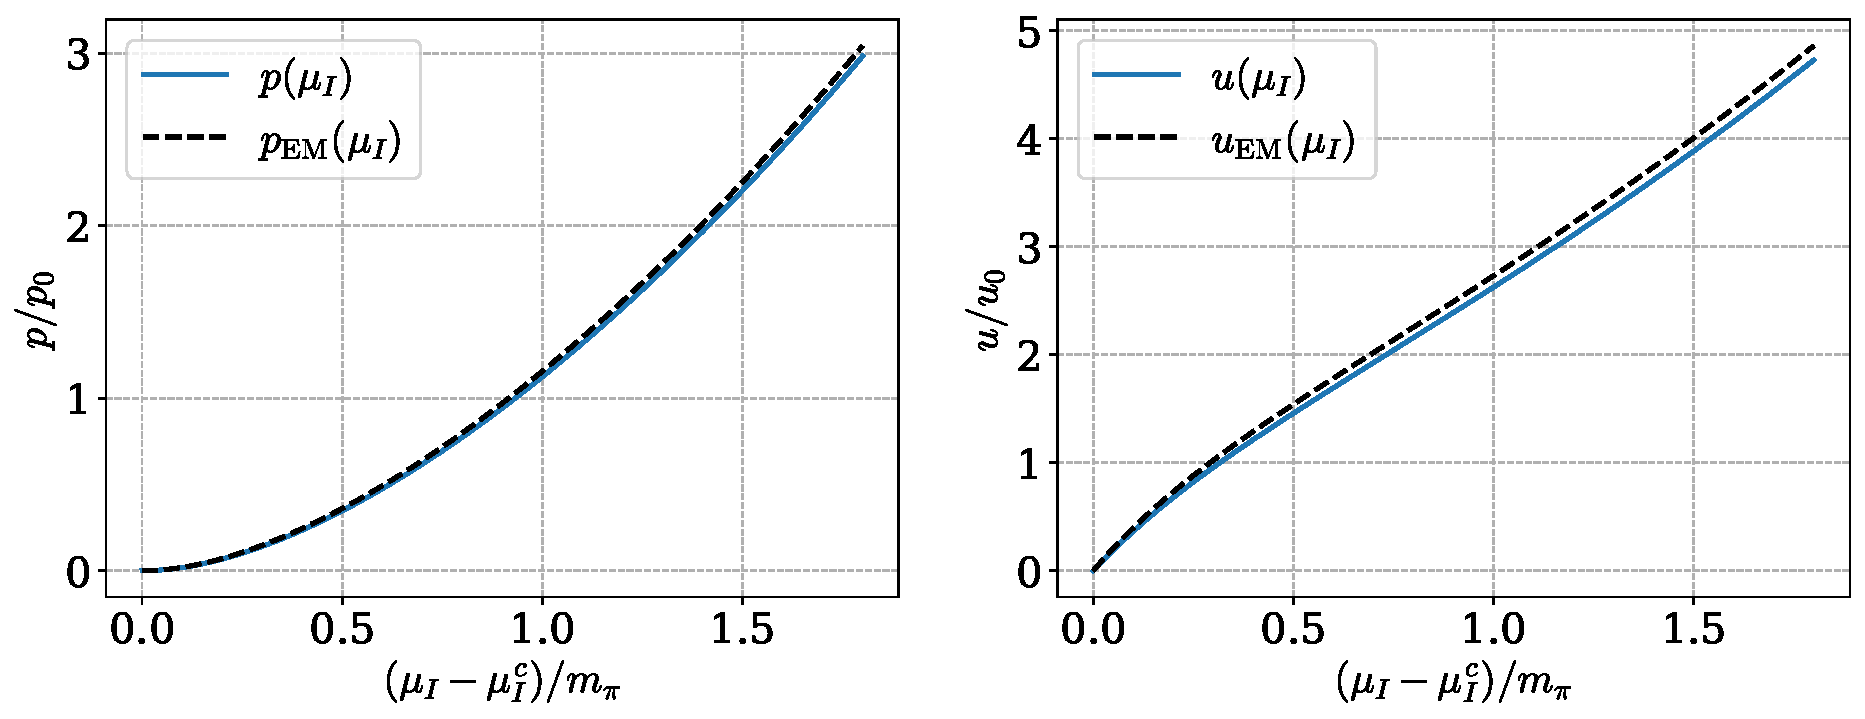
\includegraphics[width=0.95\textwidth]{../scripts/figurer/pion_star/pion_up.pdf}
    \caption{
        Left: The pressure, normalized to $p_0$, as a function of the chemical potential above the critical value, normalized to $\bar m$.
        Right: The energy density, normalized to $u_0$, also as a function of the chemical potential.
        Results with electromagnetic interaction are shown as dashed lines.
        The $y$-axis corresponds to different absolute values of isospin-chemical potential, as the critical value of the chemical is changed by the inclusion of electromagnetic interactions, see main text for details.
        }
        \label{fig: pressure and energy with EM interaction}
\end{figure}



\begin{figure}[!htb]
    \centering
    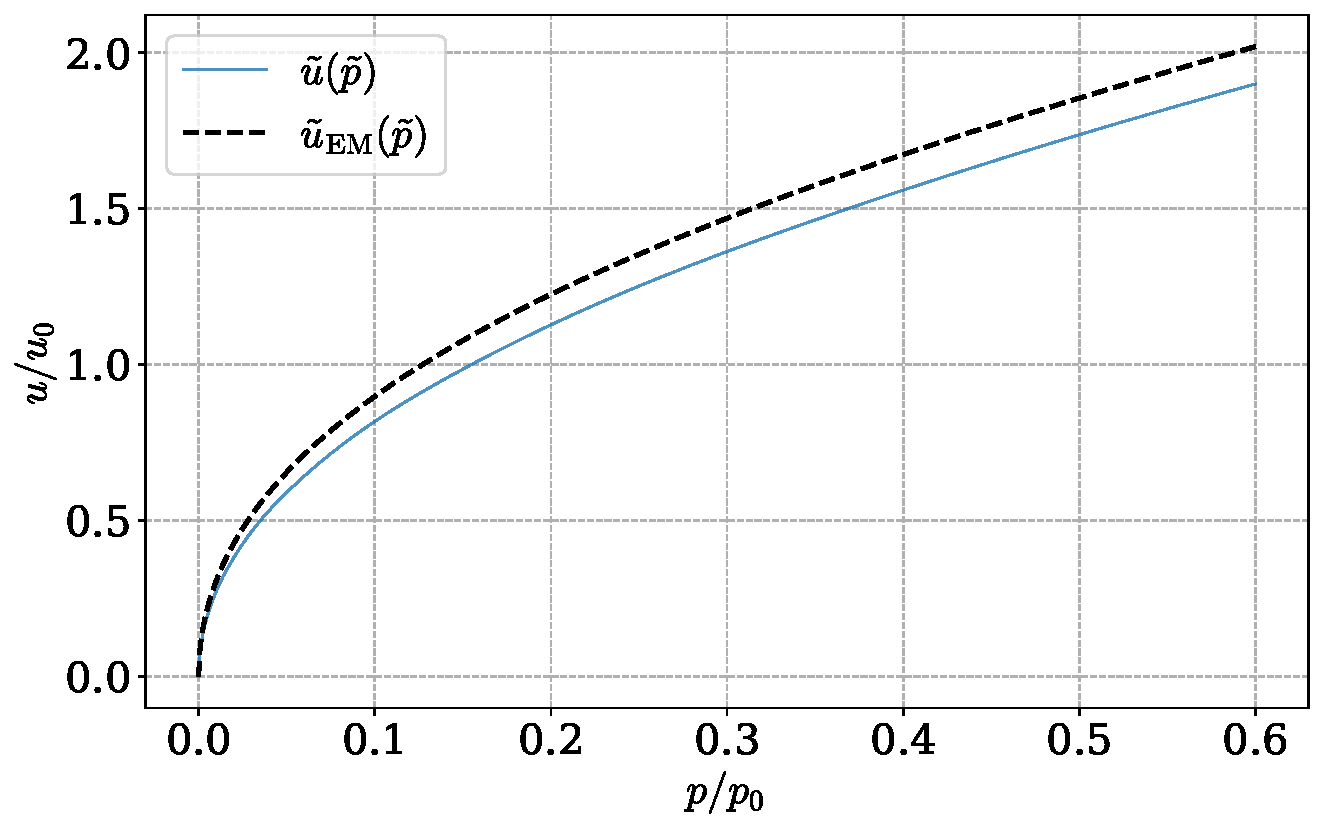
\includegraphics[width=0.65\textwidth]{../scripts/figurer/pion_star/pion_eos_EM.pdf}
    \caption{
        The equation of state in the pion condensate phase. 
        Results with electromagnetic interactions are shown as dashed lines.
        The energy density and pressure is normalized to $u_0$ and $p_0 = u_0$.
        }
    \label{fig: eos chpt em interaction}
\end{figure}





\section{Phase transitions}

As the static Lagrangian has the same form in the kaon condensate phase, the analysis will be the same.
The system will be in the phase whose static Lagrangian minimizes the free energy, or equivalently maximizes the pressure.
We can therefore find the transition line between the condensates by setting pressure of the two condensates equal.
Using \autoref{pressure leading order chpt}, and the similar expression in the kaon condensate, we get
%
\begin{equation}
    p 
    = \frac{1}{2} f^2 m_\Kpm^2 \left( \frac{\mu_\Kpm}{m_\Kpm} - \frac{m_\Kpm}{\mu_\Kpm} \right)^2
    =
    \frac{1}{2} f^2m_\pi^2  \left( \frac{\mu_I}{m_\pi} - \frac{m_\pi}{\mu_I} \right)^2.
\end{equation}
%
Solving for $\mu_\Kpm$, we get
%
\begin{equation}
    \label{transition line pion and charged condensates}
    \mu_\Kpm =\frac{1}{2\mu_I} \left(\mu_I^2 - m_\pi^2  + \sqrt{(\mu_I^2 - m_\pi^2)^2 + 4\mu_I^2 m_\Kpm^2}\right).
\end{equation}
%
The transitions into the condensates are at $\mu_I = m_\pi$, and $\mu_\Kpm = m_\Kpm$.
This point, $(\mu_I, \mu_S) = (m_\pi, m_\Kpm - m_\pi/2)$, satisfies \autoref{transition line pion and charged condensates}, and is thus a triple point between the normal phase, $\pipm$ condensate and the $\Kpm$ condensate. 

Similarly, the line between the charged and neutral kaon condensed phase is defined by
%
\begin{equation}
    \frac{1}{2} f^2 m_\Kpm^2 \left( \frac{\mu_\Kpm}{m_\Kpm} - \frac{m_\Kpm}{\mu_\Kpm} \right)^2
    =
    \frac{1}{2} f^2 m_\Ko^2 \left( \frac{\mu_\Ko}{m_\Ko} - \frac{m_\Ko}{\mu_\Ko} \right)^2.
\end{equation}
%
The solution is
%
\begin{equation}
    2 \mu_\Kpm 
    = \frac{1}{\mu_\Ko}
    \left(
        \mu_\Ko^2 - m_\Ko^2  + \sqrt{(\mu_\Ko^2 - m_\Ko^2)^2 + 4\mu_\Ko^2m_\Kpm^2}
    \right).
\end{equation}
%
We can expand this to first order in the difference in mass between the kaons, $m_\Ko^2 - m_\Kpm^2 = \Delta m^2$, which gives
%
\begin{align}
    \nonumber
    \mu_\Kpm
    &= \frac{1}{\mu_\Ko} 
    \left(
        \mu_\Ko^2 - m_\Ko^2 + \sqrt{(\mu_\Ko^2 + m_\Ko^2)^2 + 4\mu_\Ko^2 \Delta m^2}
    \right)\\
    &= \mu_\Ko \left(1 + \frac{\Delta m^2}{\mu_\Ko^2 + m_\Ko^2}\right)
    + \Oh\left( \frac{\Delta m^4}{ (\mu_\Ko^2 + m_\Ko^2)^2} \right)
\end{align}
%
This is an excellent approximation, as $\Delta m^4 / m_\Ko^4 \approx 4 \times 10^{-4}$.
The triple point is in this case at $\mu_\Kpm = m_\Kpm$, $\mu_\Ko = m_\Ko$ or $(\mu_I, \mu_S) = (m_\Kpm - m_\Ko, [m_\Kpm+m_\Ko]/2)$.
If we consider $\Delta m = 0$, then this reduces to $ \mu_\Kpm = \mu_\Ko$, or $\mu_S = 0$, as obtained in~\autocite{kogutQCDSmallNonzero2001}.
Similar analysis gives the transition line between all phases.
\autoref{fig: phase diagram} shows the phase diagram in the $\mu_I-\mu_S$-plane.

\begin{figure}[!htb]
    \centering
    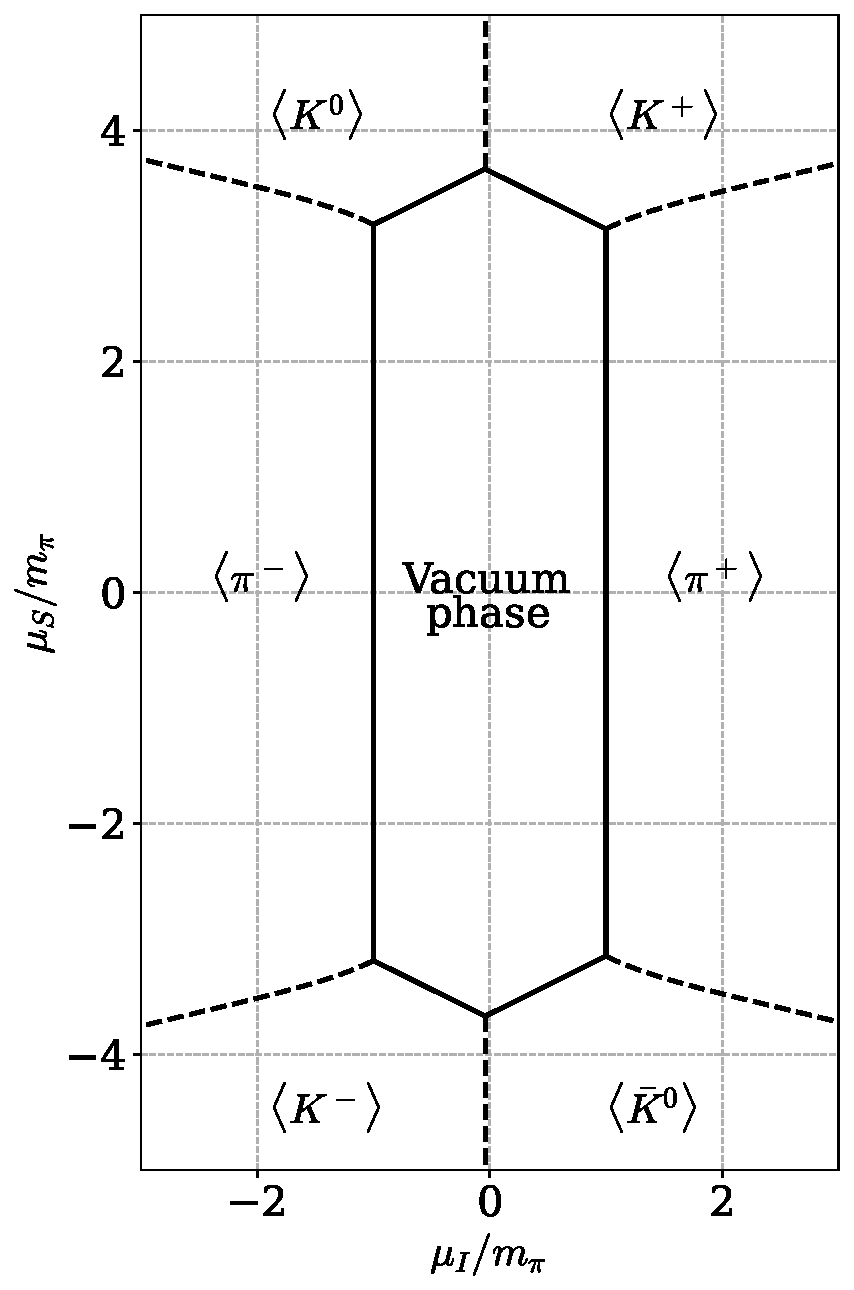
\includegraphics[width=0.5\textwidth]{../scripts/figurer/phase_diagram.pdf}
    \caption{
        The phase diagram of \chpt\ in the $\mu_I-\mu_S$-plane.
        Chemical potentials are given in units of then pion mass.
        The expectation values in each region indicate which particles form a condensate.
        The dashed lines are first-order phase transitions between the condensates, while the solid line indicates the second-order phase transition from the normal phase of the vacuum to the condensates.
        }
    \label{fig: phase diagram}
\end{figure}


As we have seen, physical quantities such as the pressure and various densities are given by the free energy minimizing state.
At the line of phase transition, this changes.
In the pion phase, the isospin and strangeness densities are
%
\begin{equation}
    n_I = - \pdv{\Eff}{\mu_I} = \mu_I \left( 1 - \frac{m_\pi^4}{\mu_I^4} \right), \quad
    n_S = - \pdv{\Eff}{\mu_S} = 0.
\end{equation}
%
In the charged kaon condensate, they are
%
\begin{equation}
    n_I = - \pdv{\Eff}{\mu_I} = 2 \pdv{\Eff}{\mu_\Kpm}
    = 2\mu_\Kpm \left( 1 - \frac{m_\Kpm^4}{\mu_\Kpm^4} \right), \quad
    n_S = - \pdv{\Eff}{\mu_S} = \mu_\Kpm \left( 1 - \frac{m_\Kpm^4}{\mu_\Kpm^4} \right).
\end{equation}
%
At the line of phase transition, $\mu_\Kpm > m_\Kpm$.
The strangeness density thus jumps discontinuously to a non-zero value.
This phase transition is therefore of first order.
In the neutral kaon condensate, the isospin density is
%
\begin{equation}
    n_I = - \pdv{\Eff}{\mu_I} = -2 \pdv{\Eff}{\mu_\Kpm}
    = - 2 \mu_\Kpm \left( 1 - \frac{m_\Kpm^4}{\mu_\Kpm^4} \right).
\end{equation}
%
This too will change discontinuously between the two kaon condensates.
Similar arguments hold between all condensates, so phase transitions between condensates are of first order.


\subsection{Electromagnetic contribution}

As we found in \autoref{subsection: including electromagnetism lo eos}, the effect of the electromagnetic interaction is to modify the isospin chemical potential by $\mu^2_I \rightarrow \mu^2_I + \Delta m_\text{EM}^2$ in all expressions.
From the structure of the Lagrangian \autoref{static lagragniang three-flavor EM kaon}, the same will happen in the case of the charged kaon, only the change will be $\mu^2_\Kpm \rightarrow \mu^2_\Kpm + \Delta m_\text{EM}^2$, while from \autoref{static lagrangian neutral kaon} we see that the results will be unchanged by electromagnetic interactions.
We define the effective chemical potential by ${\mu'}^2 = \mu^2 - \Delta_Em^2$
The transitions between the normal phase and the condensed phase will now be $\mu'_I = \bar m$ and $\mu_\Kpm' = m_\Kpm$.
The line between the pion condensed phase and the charged kaon condensed phase is now
%
\begin{equation}
    m_\Kpm^2
    \left(
         \frac{{\mu_\Kpm'}}{m_\Kpm}
         - \frac{m_\Kpm}{{\mu_\Kpm'}^2} 
        \right)^2
    =
    m_\pi^2  
    \left( 
        \frac{{\mu_I'}}{m_\pi}
        - \frac{m_\pi}{{\mu_I'}^2}  
    \right)^2,
\end{equation}
%
\begin{figure}[!htb]
    \centering
    \begin{subfigure}{0.49\textwidth}
        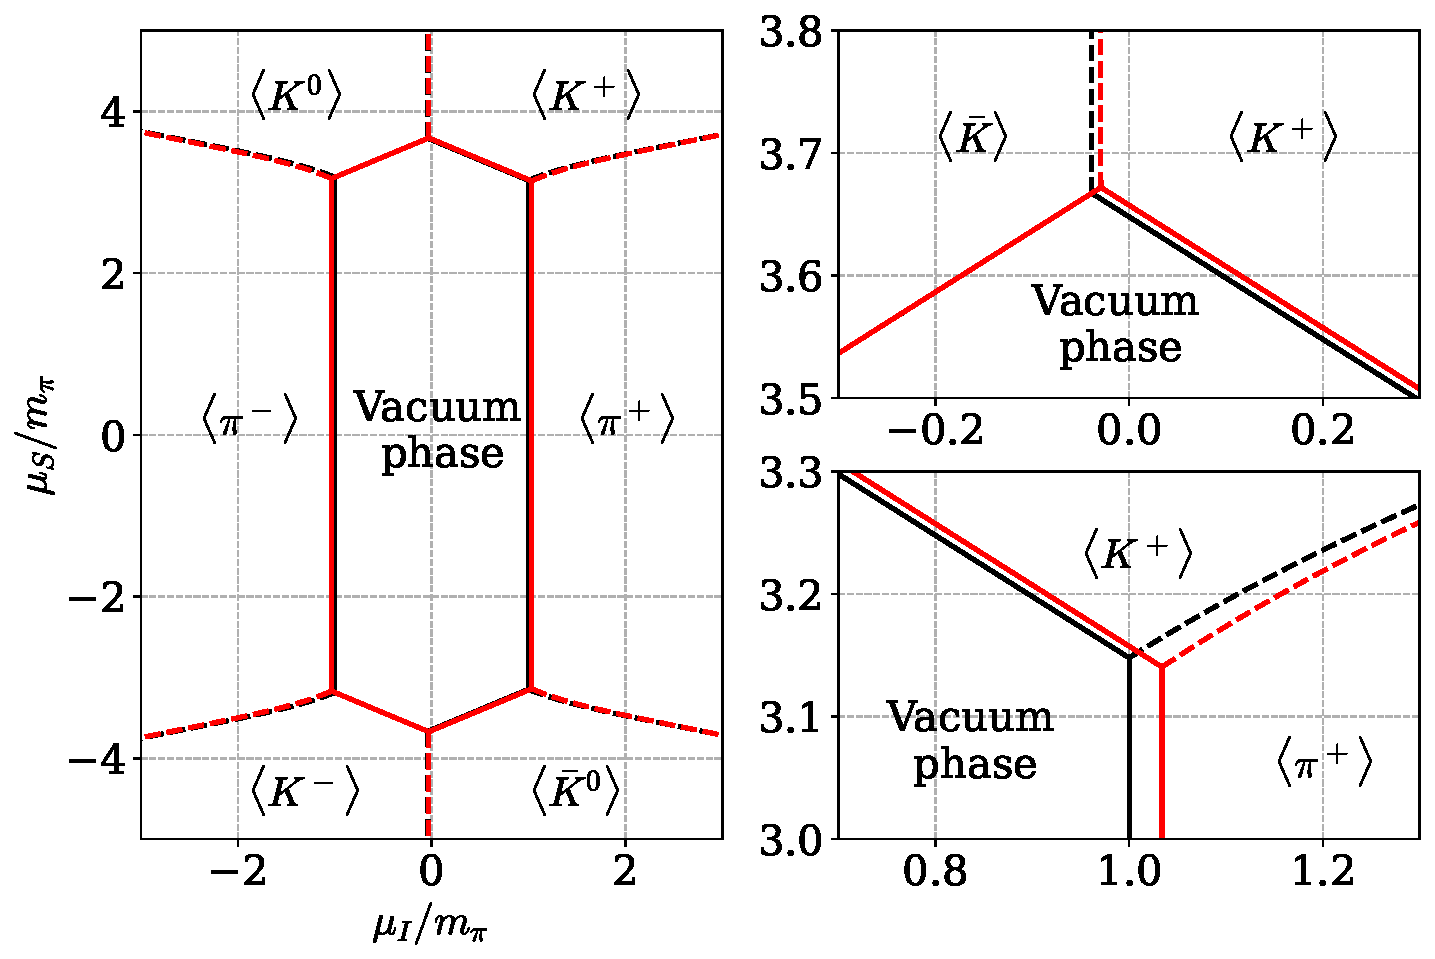
\includegraphics[width=\textwidth]{../scripts/figurer/phase_diagram_EM.pdf}
    \end{subfigure}
    \begin{subfigure}{0.49\textwidth}
        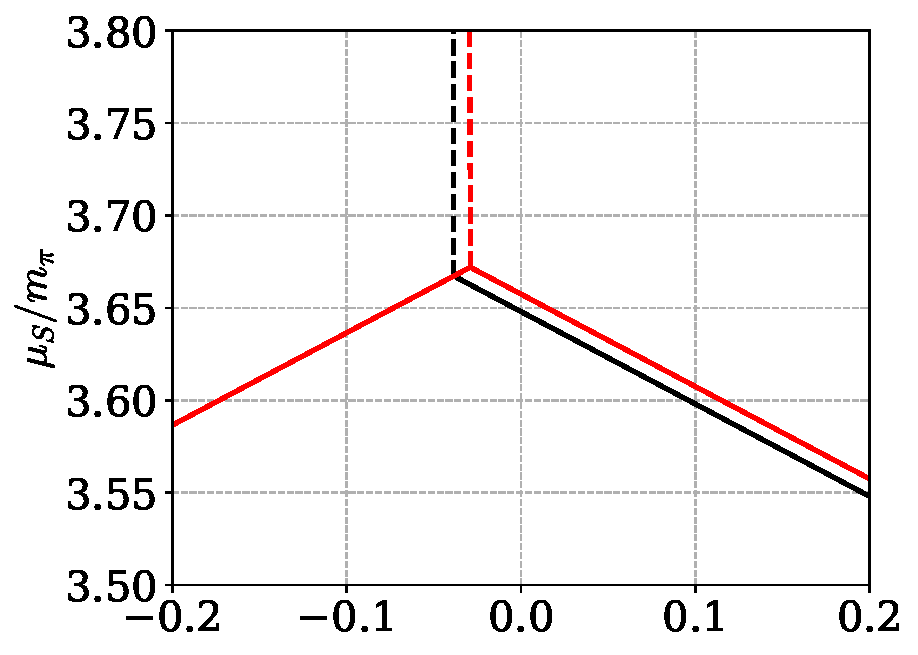
\includegraphics[width=\textwidth]{../scripts/figurer/phase_diagram_EM3.pdf}
        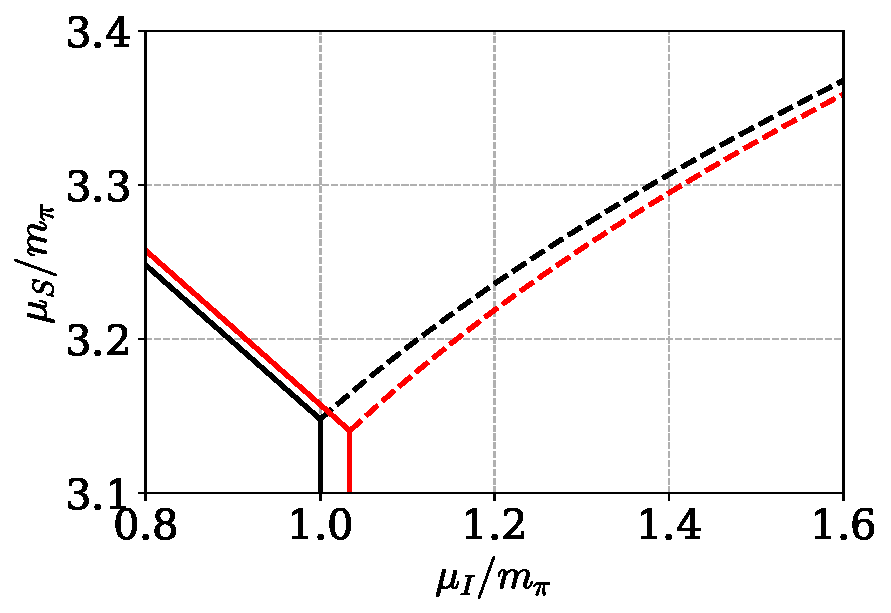
\includegraphics[width=\textwidth]{../scripts/figurer/phase_diagram_EM2.pdf}
    \end{subfigure}
    \caption{
        The phase diagram of \chpt\ in the $\mu_I-\mu_S$-plane.
        The red lines are including electromagnetic interactions, while the black are without it.
        To the right we have zoomed in on two of the triple points.
        }
    \label{fig: phase diagram EM}
\end{figure}



\section{NLO analysis}

The one-loop contribution to the free energy density is
%
\begin{equation}
    \label{one loop free energy}
    \Eff^{(1)}
    = - \frac{i}{V T} \frac{1}{2}
    \Tr{\ln\left( -\fdv{S[\pi = 0]}{\pi_a(x), \pi_b(y)} \right)}.
\end{equation}
%
This can be evaluated using the rules for functional differentiation given in \autoref{appendix: Functional derivatives}.
To leading order,
%
\begin{align}
    \fdv{S[\pi = 0]}{\pi_a(x), \pi_b(y)}
    = \fdv{}{\pi_a(x), \pi_b(y)}
    \int \dd^4 x \, \Ell^{(2)}_2
    = D_{ab}^{-1}(x - y).
\end{align}
%
Here, $\Ell^{(2)}_2$ is the quadratic part of the Lagrangian, as given in \autoref{quadratic lagrangian}, and $D^{-1}$ is the corresponding inverse propagator of the pion fields,
\begin{equation}
    D_{ab}^{-1}(x-y) = 
    \left[
        - \delta_{ab}(\partial_x^2 + m^2_a)
        + m_{12}(\delta_{a1} \delta_{b2} - \delta_{a2}\delta_{b1}) \partial_{x, 0}
    \right] \delta(x-y)
\end{equation}
%
The inverse propagator is a matrix, which means that the determinant in \autoref{one loop free energy} is both a matrix determinant, over the three pion indices, and a functional determinant.
In \autoref{section: propagator} we found the matrix part of the determinant in momentum space, which we can write using the dispersion relations of the pion fields
\begin{equation}
    \det(- D^{-1}) = \det(-p_0^2 + E_0^2) \det(-p_0^2 + E_+^2) \det(-p_0^2 + E_-^2).
\end{equation}
%
These dispersion relations are functions of the three-momentum $\vec p$, and are given in \autoref{dispresion relation pi 0} and \autoref{dispresion relation pi pm}.
The functional determinant can therefore be evaluated as
%
\begin{align}
    \nonumber
    \Tr{\ln\left( -\fdv{S[\pi = 0]}{\pi_a(x), \pi_b(y)} \right)}
    & = \ln \det(-p_0^2 + E_0^2) + \ln \det(-p_0^2 + E_+^2) + \ln \det(-p_0^2 + E_-^2) \\
    \nonumber
    & = \Tr{ \ln(-p_0^2 + E_0^2) + \ln(-p_0^2 + E_+^2)+  \ln(-p_0^2 + E_-^2) } \\
    & = (VT) \int \frac{\dd^4 p}{(2 \pi)^4} 
    \left[ \ln(-p_0^2 + E_0^2) + \ln(-p_0^2 + E_+^2) + \ln(-p_0^2 + E_-^2)  \right],
\end{align}
%
where we have used the identity $\ln\det M = \Tr \ln M $.
These terms all have the form
%
\begin{equation}
    \label{free energy logarithmic integral}
    I = \int \frac{\dd^4 p}{(2 \pi)^2} \ln(-p_0^2 + E^2),
\end{equation}
%
where $E$ is some function of the 3-momentum $\vec p$, but not $p_0$.
We use the trick
%
\begin{equation}
    \pdv{}{\alpha} \left(-p_0^2 + E^2\right)^{-\alpha} \Big|_{\alpha=0}
    = \pdv{}{\alpha} \exp {-\alpha \ln\left(- p_0^2 + E^2\right)} \Big|_{\alpha=0}
    = \ln\left(- p_0^2 + E^2\right),
\end{equation}
%
and then perform a Wick-rotation of the $p_0$-integral to write the integral on the form 
%
\begin{equation}
    I = i \pdv{}{\alpha} \int \frac{\dd^4 p}{(2 \pi)^4} \left(p_0^2 + E^2\right)^{-\alpha} \Big|_{\alpha=0},
\end{equation}
%
where $p$ now is a Euclidean four-vector.
The $p_0$ integral equals $\Phi_1(E, 1, \alpha)$, as defined in \autoref{def dimreg integral}. 
The result is therefore given by \autoref{result dimreg},
%
\begin{equation}
    \int \frac{\dd p_0}{2 \pi} (p_0^2 + E)^{-\alpha} 
    = \frac{E^{1-2\alpha}}{\sqrt{4 \pi}} \frac{\Gamma(\alpha-\frac{1}{2})}{\Gamma(\alpha)}.
\end{equation}
%
The derivative of the Gamma function is $\Gamma'(\alpha) = \psi(\alpha)\Gamma(\alpha)$, where $\psi(\alpha)$ is the digamma function.
Using
%
\begin{align}
    \pdv{}{\alpha} & \frac{\Gamma(\alpha - \frac{1}{2}) }{\Gamma(\alpha)} \Big|_{\alpha=0}
    = \Gamma\left(\alpha - \frac{1}{2}\right) \frac{\psi(\alpha - \frac{1}{2}) - \psi(\alpha)}{\Gamma(\alpha)} \Big|_{\alpha=0}
    = \sqrt{4 \pi}, \\
    & \frac{\Gamma(\alpha - \frac{1}{2}) }{\Gamma(\alpha)}\Big|_{\alpha=0} = 0,
\end{align}
%
we get
%
\begin{equation}
    I = i \int \frac{\dd^3 p}{(2 \pi)^3} E.
\end{equation}
%
We see that the result is what we would expect physically; the total energy is the integral of each mode's energy.
This also agrees with the result from \autoref{appendix: thermal field theory} in the zero-temperature limit $\beta \rightarrow \infty$.
The one-loop contribution can therefore be written
%
\begin{equation}
    \Eff^{(1)} = 
    \frac{1}{2} 
    \left[\int \frac{\dd^3 p}{(2\pi)^3} E_0 + \int  \frac{\dd^3 p}{(2\pi)^3} (E_+ + E_-)\right]
    = \Eff^{(1)}_{\pi_0} +\Eff^{(1)}_{\pi_\pm}.
\end{equation}
%
The first integral is identical to what we find for a free field in \autoref{section:free scalar field}, in the zero-temperature limit.
These terms are all divergent and must be regularized.
We will use dimensional regularization, in which the integral is generalized to $d$ dimensions, and the $\overline{\mathrm{MS}}$-scheme, as described in \autoref{section: regualting free energy}.
Using the result for a free field \autoref{free field regularized energy}, we get
%
\begin{equation}
    \label{Free energy pi 0}
    \Eff^{(1)}_{\pi_0} 
    = 
    - \mu^{-2 \epsilon}  \frac{1}{4} \frac{m_3^4}{(4\pi)^2} 
    \left( \frac{1}{\epsilon} + \frac{3}{2} + \ln \frac{\tilde \mu^2}{m_3^2} \right)
    + \mathcal{O}(\epsilon),
\end{equation}
%
where $\mu$ is the renormalization scale, a parameter with mass-dimension 1, introduced to ensure the action integral remains dimensionless during dimensional regularization.
$\tilde \mu$ is a related to $\mu$ as described in \autoref{definition mu tilde MS bar}.

The contribution to the free energy from the $\pi_+$ and $\pi_-$ particles is more complicated, as the dispersion relation is given by
%
\begin{equation}
    E_\pm
    = 
    \sqrt{
        |\vv p|^2 +
        \frac{1}{2}
        \left(
            m_1^2 + m_2^2 + m_{12}^2 
        \right)
        \pm 
        \frac{1}{2}
        \sqrt{
            4|\vv p|^2m_{12}^2 
            +
            \left(
                m_1^2 + m_2^2 + m_{12}^2
            \right)^2
            - 4 m_1^2 m_2^2
        }
    }.
\end{equation}
%
This is not an integral we can easily do in dimensional regularization.
Instead, we will seek a function $f(|\vv p|)$ with the same UV-behavior, that is, behavior for large $\vv p$, as $E_+ + E_-$.
If we then add $0 = f(|\vv p|) - f(|\vv p|)$ to the integrand, we can isolate the divergent behavior
%
\begin{equation}
    \Eff_{\pi_\pm}^{(1)}
    = 
    \frac{1}{2} \int \frac{\dd^3 p}{(2\pi)^3} [E_+ + E_- + f(|\vv p|) - f(|\vv p|)]
    = \Eff^{(1)}_{\mathrm{fin}, \pi_\pm } + \Eff^{(1)}_{\mathrm{div}, \pi_\pm}.
\end{equation}
%
This results in a finite integral,
%
\begin{equation}
    \Eff^{(1)}_{\mathrm{fin}, \pi_\pm } = \frac{1}{2} \int \frac{\dd^3 p}{(2\pi)^3} [E_+ + E_- - f(|\vv p|)],
\end{equation}
%
which we can evaluate numerically, and a divergent integral
%
\begin{equation}
    \Eff^{(1)}_{\mathrm{div}, \pi_\pm }
    = 
    \frac{1}{2} \int \frac{\dd^3 p}{(2\pi)^3} f(|\vv p|),
\end{equation}
%
which we hopefully will be able to do in dimensional regularization.
We can explore the UV-behavior of $E_+ + E_-$ by expanding it in powers of $1 / \abs{\vv{p}}$,
%
\begin{align}
    \nonumber
    E_+ + E_-
    & = 
    2  \abs{\vv{p}}
    + \frac{m_{12} + 2(m_1^2 + m_2^2)}{4} \, {\abs{\vv{p}}}^{-1}
    - \frac{m_{12}^4 + 4 m_{12}^2(m_1^2 + m_2^2) + 8(m_1^4 + m_2^4)}{64}
    {\abs{\vv{p}}}^{-3}
    + \Oh (\abs{\vv{p}}^{-5})
    \\
    & = 
    a_1  \abs{\vv{p}}
    + a_2 \, {\abs{\vv{p}}}^{-1}
    + a_3
    {\abs{\vv{p}}}^{-3}
    + \Oh (\abs{\vv{p}}^{-5}).
\end{align}
%
We have defined new constants $a_i$ for brevity of notation.
As
%
\begin{equation}
    \int_{\R^3} \frac{\dd^3 p}{(2 \pi)^3} |\vv p|^{n}
    = C \int_{0}^\infty \dd p \, p^{2 + n}
\end{equation}
%
is UV divergent for $n \geq -3$, $f$ need to match the expansion of $E_+ + E_-$ up to and including $\Oh(|\vv{p}|^{-3})$ for $\Eff^{(1)}_{\mathrm{fin}, \pi_\pm }$ to be finite.
The most obvious choice for $f$ is
%
\begin{equation}
    f(|\vv p|) 
    = a_1  \abs{\vv{p}} + a_2 \, {\abs{\vv{p}}}^{-1} + a_3 \, {\abs{\vv{p}}}^{-3}.
\end{equation}
%
However, this introduces a new problem.
$f$ has the same UV-behavior as $E_+ + E_-$, but the last term diverges in the IR, that is, for low $|\vv p|$.
This can be amended by introducing a mass term.
Let
%
\begin{equation}
    |\vv p|^{-3} 
    = 
    \left(\frac{1}{\sqrt{|\vv p|^2}}\right)^3 
    \longrightarrow 
    \left(\frac{1}{\sqrt{|\vv p|^2 + m^2}}\right)^3.
\end{equation}
%
For $|\vv p|^2 \rightarrow \infty$, this is asymptotic to $|\vv p|^{-3}$, so it retains its UV behavior.
However, for $|\vv p| \rightarrow 0$, it now approaches $m^{-3}$, so the IR-divergence is gone.
The cost of this technique is that we have introduced an arbitrary mass parameter.
Any final result must thus be independent of the value of $m$ to be acceptable.

We will instead regularize the integral by defining $E_i = \sqrt{|\vv{p}|^2 + \tilde m_i^2}$, and $\tilde m_i^2 = m_i^2 + \frac{1}{4} m_{12}^2$.
Using the definition of the masses, \autoref{m1}, \autoref{m2}, \autoref{m3}, and \autoref{m12}, we get
%
\begin{align}
    m_3^2 & = \bar m^2 \cos \alpha + \mu_ I^2 \sin^2 \alpha, \\
    \label{tilde m1}
    \tilde m_1^2 
    & 
    = m_1^2 + \mu^2 \cos\alpha^2
    = \bar m^2 \cos \alpha + \mu_I^2 \sin^2 \alpha
    = m_3^2 \\
    \label{tilde m2}
    \tilde m_2^2 
    & = m_2^2 + \mu^2 \cos\alpha^2
    = \bar m^2 \cos \alpha.
\end{align}
%
Finally, we define $f(|\vv p|) = E_1 + E_2$, which differ from $E_+ + E_-$ by $\Oh\left(|\vv p|^{-5}\right)$ and is well-behaved in the IR.
This leads to a divergent integral the same form as in the case of a free scalar.
Thus, in the $\mathrm{\overline{MS}}$-scheme, 
%
\begin{equation}
    \Eff^{(1)}_{\mathrm{div}, \pi_\pm }
    =
    - \mu^{-2 \epsilon} \frac{1}{4} \frac{\tilde m_1^4}{(4\pi)^2} 
    \left(
        \frac{1}{\epsilon} + \frac{3}{2} + \ln \frac{\tilde \mu^2}{\tilde m_1^2}
    \right) 
    -  \mu^{-2 \epsilon} \frac{1}{4} \frac{\tilde m_2^4}{(4\pi)^2} 
    \left(
        \frac{1}{\epsilon} + \frac{3}{2} + \ln \frac{\tilde \mu^2}{\tilde m_2^2}
    \right) 
    + \mathcal{O}(\epsilon).
\end{equation}
%
We define
%
\begin{equation}
    \Eff^{(1)}_{\mathrm{fin}, \pi_\pm}
    = 
    \frac{1}{2} \int \frac{\dd^3 p}{(2\pi)^3} (E_+ + E_- - E_1 - E_2),
\end{equation}
%
which is a finite integral.
The total one-loop contribution is then, using \autoref{tilde m1} and \autoref{tilde m2},
%
\begin{align}
    \Eff^{(2)}
    & = 
    \Eff^{(1)}_{\mathrm{fin}, \pi_\pm}
    - \mu^{-2 \epsilon} \frac{1}{2}\frac{1}{(4\pi)^2}
    \left[
        \left( \frac{1}{\epsilon} + \frac{3}{2} + \ln \frac{\tilde \mu^2}{m_3^2 } \right)
        m_3^4
        +
        \frac{1}{2}
        \left( \frac{1}{\epsilon} + \frac{3}{2} + \ln \frac{\tilde \mu^2}{\tilde m_2^2} \right)
        \tilde m_2^4
    \right]
    + \Oh(\epsilon).
\end{align}

